\chapter{Propuesta de Solución}
El análisis de las distintas alternativas disponibles para mejorar el rendimiento de la interfaz de red efectuado en el capítulo anterior nos motiva a diseñar e implementar una propuesta de solución que satisfaga ciertos requerimientos puntuales, en pos de ubicarla como una opción viable de uso en entornos como el propuesto.

En el presente capítulo se formalizan los requerimientos mínimos que constituyen nuestra solución ideal. A continuación se desarrolla un modelo para esquematizar el funcionamiento de la solución propuesta y se describe la implementación de la misma, para terminar con una evaluación final de performance bajo los mismos entornos que las pruebas desarrolladas a lo largo de la presente investigación.

\section{Formalización de Requerimientos}
Como se ilustró en el capítulo anterior, las distintas soluciones disponibles para mejorar la performance de las estructuras sockets en el kernel de Linux se caracterizan por ser complejas en su funcionamiento ya sea por su implementación para funcionar sobre aplicaciones ya desplegadas en un sistema, o por quebrantar ciertos principios de programación definidos -como los sugeridos por el modelo estándar OSI- con consecuencias como tener que modificar el codigo de programas perfectamente operativos bajo el modelo tradicional. El objetivo en este punto es caracterizar las especificaciones ideales que debe satisfacer un desarrollo de optimización de la operación de los sockets en el marco de la preservación de caracteristicas deseadas, especificadas por el ya mencionado modelo OSI.

En función de lo anterior, a continuación se especifican las propiedades estructurales que debe contemplar una solución ideal:


\begin{description}
\item[Rendimiento] El requerimiento principal para la solución objetivo constituye el garantizar un buen rendimiento. La solución debe poder brindar tiempos -a lo menos- competitivos con la mejor alternativa evaluada a lo largo de la investigación en curso, que corresponde al rendimiento obtenido con el mecanismo de \emph{ReusePort}.
\item[Bajo Overhead] A fin de lograr una solución con bajo overhead e impacto con el resto del sistema, se debe procurar considerar una alternativa que opere en los niveles más bajos del sistema operativo -A nivel de Kernel idealmente- a fin de evitar la sobrecarga efectuada por concepto de interrupciones y call-chains ???? que son propias de soluciones que operan en espacio de usuario.
\item[Modularidad] El esquema ideal debe ser modular en el sentido de garantizar una sencilla instalación y remoción de la misma en un sistema, sin necesitar significativas dependencias de otros componentes. En otra arista de este mismo requerimiento, se busca desarrollar una solución que permita modificarciones en sí misma de manera sencilla a fin de garantizar \textbf{extensibilidad}.
\item[Adaptabilidad] Finalmente, una propiedad que debe contemplar la solución es ser facilmente configurable y adaptable a los distintos entornos y requerimientos que se presenten en línea con las necesidades de rendimiento que se persigan.
\end{description}

Las características antes mencionadas sirven como requerimientos estructurales en lo que se postula como nuestra propuesta de diseño de solución.

\section{Modelo de Funcionamiento de la Solución}
Tomando en consideración los requerimientos descritos en la sección anterior, se optó por una solución cuyo modelo de funcionamiento fuese como el descrito en la imagen \ref{modeloUDPRedistribuyeModule}, construido como un módulo del kernel que sea capaz de intervenir paquetes de Internet de las características que atañen éste estudio, y los redistribuyan entre un pool de nuevos puertos. Para una primera versión de ésta solución se postularon 2 esquemas de distribución que se describen en apartados posteriores.

IMAGEN

Ésta desición de diseño se fundamenta en que, con éste enfoque se satisfacen casi todos los requerimientos definidos en la sección anterior: En primer lugar, es un enfoque que añade \textbf{bajo overhead} al sistema, al ser un módulo que se ejecuta en el espacio del Kernel, por lo que cuenta con privilegios que evitan la sobrecarga experimentada por soluciones en espacio usuario. Segundo, siendo un módulo, al momento de instalarlo en el sistema se pueden realizar todas las \textbf{configuraciones} pertinentes, permitiendo un grado de adaptabilidad de acuerdo al entorno y resultado deseado. En tercer lugar, al ser un módulo, es facilmente \textbf{modificable} permitiendo añadir, modificar o eliminar del mismo, reglas definidas o esquemas de distribución. Basta modificarlo, recompilarlo y está listo para operar. Por lo mismo, es facilmente removible del sistema y no guarda ningúna dependencia estricta de terceros.

Las componentes que rigen el modelo en su operación ilustrados en la imagen \ref{modeloUDPRedistribuyeModule} se describen como:

\begin{description}
\item[hook\_port] Valor que determina el puerto a interceptar para la redirección de paquetes.
\item[redirect\_port] Colección de valores que indican los puertos hacia los cuales redistribuir los paquetes interceptados y modificados.
\item[verbose] Índice del grado de detalle con que se guardarán registros de acción del módulo en los mensajes del Kernel.
\end{description}

En la práctica, la operación de la solución propuesta se inspira en el mecanismo de un \emph{proxy}, modificando sólamente los valores en las cabeceras de los paquetes intervenidos. El modelo implementa la siguiente lógica de instrucciones:

\begin{enumerate}
\item Interceptar paquetes de tipo UDP y que estén dirigidos a un determinado puerto (\textbf{hook\_port}).
\item Modificar el paquete, actualizando valores como el \emph{checksum} del mismo.
\item Redireccionar el paquete, modificando el puerto de destino del paquete (\textbf{redirect\_port}) de acuerdo al esquema de distribución operativo.
\item Reincorporación del paquete modificado en el tránsito de distribución del kernel por la vía ordinaria.
\end{enumerate}

Por su naturaleza de acción, la solución opera estrictamente entre las capas de Red y de Transporte en el modelo OSI, interviniendo esos niveles de abstracción, a través de la modificación de los encabezados correspondientes al empaquetamiento por los protocolos IP y UDP respectivamente.

\subsection{Esquemas de Distribución}
Como ya se mencionó, la solución desarrollada comprende una etapa de distribución de paquetes de acuerdo a distintos esquemas de distribución. En este contexto, un esquema de distribución lo definiremos como un conjunto de reglas para reasignar los paquetes interceptados entre un pool de puertos previamente definidos. En la versión desarrollada del \textbf{UDPRedistributeModule} se implementaron 2 esquemas de distribución: \emph{RandomSched} y \emph{SequentialSched}.

\subsubsection{RandomSched}
El esquema de distribución \emph{RandomSched} realiza una distribución entre puertos de manera aleatoria. La aleatoriedad de éste esquema se consigue por medio de la llamada de sistema \verb=get_random_bytes()= que sugiere una distribución aleatorizada de resultados y redistribuyendo los paquetes de acuerdo a la aplicación de una operación de módulo sobre el valor aleatorio, por el total de puertos blanco de redistribución. La utilización de dicha función se justifica en ser uno de los mecanismos más sencillos de obtener aleatoriedad en demanda en el espacio del Kernel y que, según su documentación, sus valores generados siguen una distribución uniforme.

\begin{figure}[th!]
\centering
\subfigure[text1]{
	
\includegraphics[width=.3\textwidth]{imagenes/fcfm}
}
\subfigure[text2]{
	
\includegraphics[width=.3\textwidth]{imagenes/fcfm}
}
\subfigure[text3]{
	
\includegraphics[width=.3\textwidth]{imagenes/fcfm}
}
\caption{Evolución en la distribución de paquetes usando el esquema aleatorio por \emph{RandomSched}.}
\label{fig:RandomSched}
\end{figure}

A pesar de que en teória éste esquema en promedio promete una distribución uniforme, en la práctica es posible que la carga no sea en efecto perfectamente distribuida, por lo que éste esquema es práctico en escenarios donde se desee cierta entropía en la reasaignación de carga entre puertos de destino.

\subsubsection{SequentialSched}
El segundo esquema de distribución diseñado es denominado \emph{SequentialSched}. En éste caso, se hace una distribución secuencial entre los distintos puertos de destino de distribución asignados en el módulo. De ésta manera, éste esquema consigue una perfecta distribución entre puertos de redirección logrando una carga equitativa entre todos ellos.

\begin{figure}[th!]
\centering
\subfigure[text1]{
	
\includegraphics[width=.3\textwidth]{imagenes/fcfm}
}
\subfigure[text2]{
	
\includegraphics[width=.3\textwidth]{imagenes/fcfm}
}
\subfigure[text3]{
	
\includegraphics[width=.3\textwidth]{imagenes/fcfm}
}
\caption{Evolución en la distribución de paquetes usando el esquema secuencial por \emph{SequentialSched}.}
\label{fig:SequentialSched}
\end{figure}

\section{Implementación}
El mecanismo de funcionamiento planetado en la sección anterior postula modificar el destino final de los paquetes, modificando el puerto de destino de los mismos. Dicha operación implica dos caracteristicas a considerar:

\begin{enumerate}
\item Interceptar paquetes en el momento apropiado. A priori dicho momento sería idealmente apenas el sistema reconozca el arribo de un paquete.
\item Modificar paquetes para su redirección. Cómo se explicó en la sección XXXXXXX, la información de puerto de destino es una especifiación propia de la \textbf{capa de transporte} según el modelo OSI, y por lo tanto, dicha información es inherente a los encabezados de dicha capa.
\end{enumerate}

Dados los requerimientos anteriores, para la implementación de la solución se optó por el diseño de un módulo del kernel operacional sobre el framework de \emph{Netfilters} ????????????, el cual permite intervenir paquetes de las características relacionadas al caso de estudio y brinda la flexibilidad para modificar los encabezados de los mismos, logrando el efecto de redistribución entre distintos puertos, y siendo lo suficientemente flexible como para emplear distintos esquemas de distribución para la redirección de los mismos. Además, al ser un módulo del kernel, existen diversas guias técnicas que profundizan los aspectos de diseño a considerar en construcción del mismo ?????????.

\subsection{NetFilter Framework}
Netfilter ???????? es un framework disponible en el núcleo de sistemas Linux que permite la manipulación de paquetes en distintos niveles del tránsito de los mismos a través del stack de protocolos de red del kernel. Para ello, Netfilters provee una interfaz para implementar los denominados \emph{hooks}, que son funciones de intervención de paquetes donde se da la libertad de programar libremente operaciones sobre cada estructura de paquete intervenido. Los \emph{hooks} implementados deben ser registrados en el sistema en un \emph{punto de intercepción} y es el mismo kernel el encargado de incluirlos en su rutina de inspección de paquetes a medida que los mismos van llegando al sistema, aplicándolos de acuerdo a reglas de prioridad y puntos de intervención bien definidos. Netfilters es una de las herramientas más potentes para la manipulación de paquetes, siendo la base de distintas herramientas que operan en espacio usuario como es \textbf{IPTables} y MASASSSSSSSSSS.

Las capacidades de manipulación que provee Netfilters son bastante poderosas, abarcando un amplio espacio de acción en el sistema, postulandose como una interesante herramienta que contemplar en el desarrollo de la solución al desafío planteado.

\subsubsection{Arquitectura de Interrupción en Netfilters}
El framework provee una arquitectura de seguimiento de los distintos paquetes para interceptar que se modela en un esquema definido en la imagen \ref{netfilterArchitecture}. Ésta arquitectura es lo suficientemente amplia como para intervenir paquetes en distintos niveles de comunicación y transito a través del kernel.

\begin{figure}[!h]
	\centering
	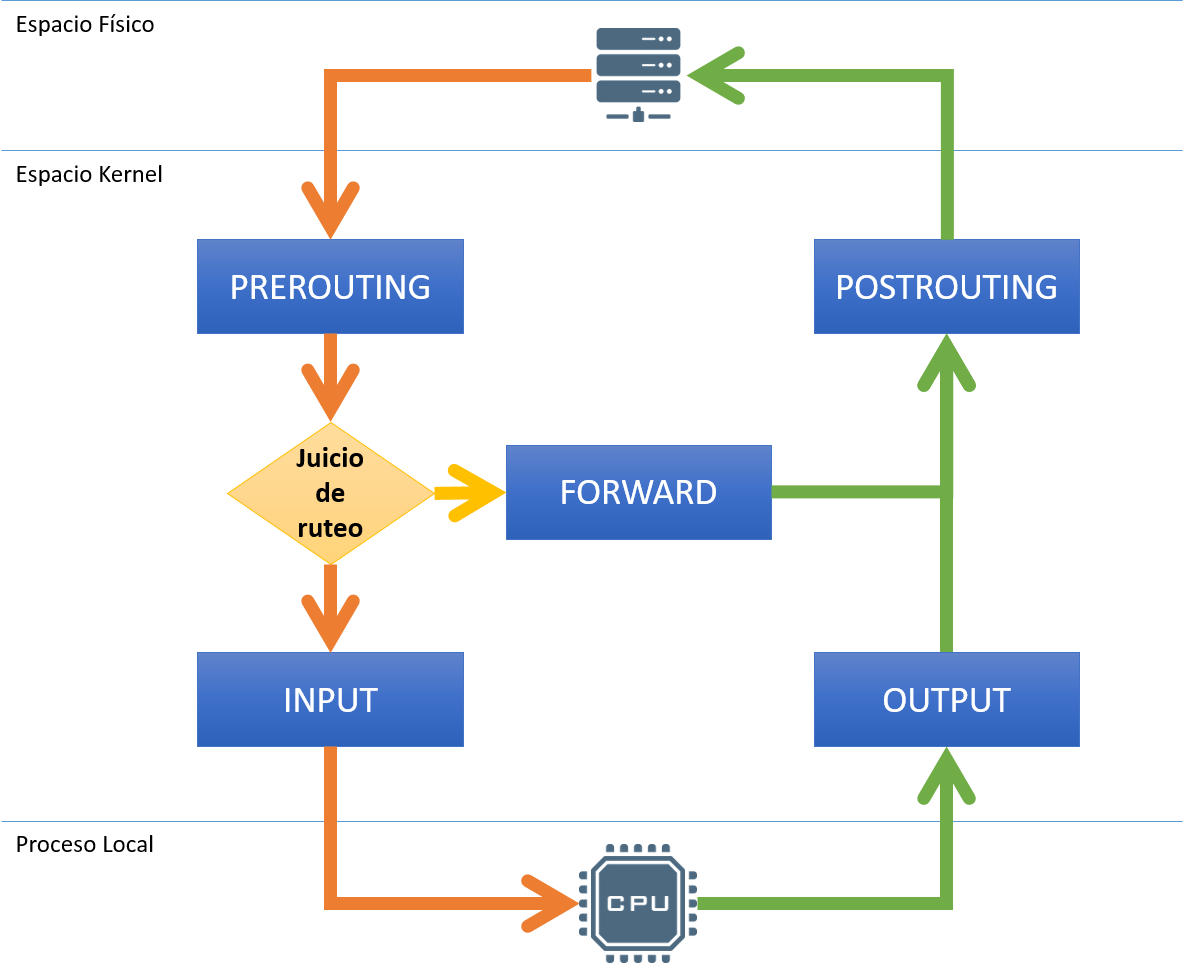
\includegraphics[scale=.5]{imagenes/netfilterArchitecture}
	\caption{Esquema de la arquitectura de interrupción disponible para la intervención de paquetes provisto por el Netfilters Framework. REVISAR EN \url{http://amsekharkernel.blogspot.cl/2012/01/what-is-netfilter-in-linux.html}}
	\label{netfilterArchitecture}
\end{figure}

El esquema ilustrado en la figura \ref{netfilterArchitecture} da cuenta del flujo que recorre un paquete en el kernel en consideración de los modos de intervención que brinda el framework de Netfilters. Cada uno de los puntos ilustrados en dicho diagrama es un potencial \emph{punto de intervención}, y da cuenta de alguna etapa en el arrivo o salida de un paquete. Los distintos puntos de intervención disponibles en \emph{IPv4} se detallan a continuación:

\begin{description}
\item[NF\_IP\_PRE\_ROUTING] Incoming packets pass this hook in \verb=ip_rcv()= before routing
\item[NF\_IP\_INPUT] All incoming packets addressed to the local host pass this hook in \verb=ip\_local\_deliver()=.
\item[NF\_IP\_FORWARD] All incoming packets not addressed to the local host pass this hook in \verb=ip_forward()=
\item[NF\_IP\_OUTPUT] All outgoing packets created by this local computer pass this hook in \verb=ip_build_and_send_pkt()=
\item[NF\_IP\_POST\_ROUTING] All outgoing packets (forwarded or locally created) will pass this hook in \verb=ip_finish_output()=
\end{description}

\subsubsection{Implementación de funciones de Interrupción usando Netfilters}

El framework en cuestión está diseñado para poder aprovechar sus funcionalidades facilmente a partir de un módulo del kernel, para ello, basta incluir las directivas de encabezados del framework en el módulo (\verb=#include <linux/netfilter.h>=) e implementar los mecanísmos de registro del \emph{hook} en el sistema, especificando sus opciones como prioridad, familia y punto de interrupción, para ello, se usan valores de constantes provistos por el mismo framework. Además de lo anterior, se debe implementar la función a aplicar sobre cada paquete intervenido, para lo cual es necesario seguir la convención que especifica el mismo framework, esto es un prototipo de función que propone el framework que se ilustra en el segmento de código ?????????????.

\definecolor{mygray}{rgb}{0.95,0.95,0.95}
\lstset{language=C,
		frame=single,
		backgroundcolor=\color{mygray}
		}
\begin{lstlisting}[caption=ESO]
static unsigned int hook_func(
            		unsigned int hooknum,
            		struct sk_buff *skb, 
            		const struct net_device *in, 
            		const struct net_device *out, 
            		int (*okfn)(struct sk_buff *));
\end{lstlisting}

Este prototipo de función comprende 5 valores a recibir que contienen información relacionada al paquete que se ha de intervenir por la función \verb=hook_func= misma. \textbf{hooknum} Que corresponde al valor del mismo nombre que se asigna al momento de registrar la función de \emph{hook} y que hace referencia al punto de interrupción en que inspeccionará paquetes nuestro \emph{hook}. \textbf{skb} que es una estructura tipo \verb=sk_buff= que almacena el paquete interceptado propiamente tal, y del cual se pueden extraer y modificar los encabezados de las capas de transporte y red para modificar el tránsito del paquete. Los punteros \textbf{in} y \textbf{out} de estruturas \verb=net_device= que se refieren a las interfaces de procedencia y destino del paquete que registra al momento de interceptarlo, Y finalmente \textbf{sk\_buff}, que se refiere a AAAAAAAAAAAAAAAAAAAAAAAAAAAAAAAAA.

Finalmente, las funciones de \emph{hook} deben especificar un valor de retorno que determina el camino a seguir por el paquete intervenido. En éste sentido, el framework especifica 5 posibles valores de retorno para las funciones de interrupción especificadas a continuación:
\begin{description}
\item[NF\_ACCEPT:] Para que el paquete prosiga su entrega, es decir, promueve el paquete a la siguiente etapa de distribución según módulo de Red del kernel.
\item[NF\_DROP:] Para descartar el paquete, cancelando su entrega.
\item[NF\_STOLEN:] Para adueñarse del paquete. Es decir, sacar el paquete del entorno de Netfilters y brindarle su propiedad a la misma función de \emph{hook}.
\item[NF\_QUEUE:] Para encolar el paquete y poder manipularlo en espacio usuario.
\item[NF\_REPEAT:] Para llamar a la función de \emph{hook} en cuestión, otra vez.
\end{description}

\subsection{Implementación de la solución usando Netfilters}
Para el proceso de registro del \emph{hook} se tomaron ciertas consideraciones que permitieran garantizar la plena operatividad de la solución en el entorno de trabajo.

En primer lugar, se seleccionó como punto de interrupción del \emph{hook} a \verb=NF_INET_PRE_ROUTING=, ello pues corresponde al nivel más temprano de interrupción desde el arribo del paquete por la interfaz del sistema que admite el framework y básicamente captura todo transito de paquetes. Por cuestiones de naturaleza de paquetes a trabajar se configuró la familia del \emph{hook} como \verb=PF_INET= que abarca a la familia de los protocolos de internet\footnote{REFERENCIAAAAAAAAAAAA} que contiene tipos útiles para la manipulación de los paquetes que son del tipo que nos interesa interceptar. Para el apartado de prioridad del \emph{hook}, que especifica el órden de ejecución los diferentes hooks programados en el sistema, se seleccionó como el valor constante \verb=NF_IP_PRI_FIRST= que provee el framework mismo y que garantiza la más pronta aplicación posible de nuestro hook a los paquetes interceptados. Ésta desición se apoya en que se desea el menor impacto para con otras componentes del sistema, por ello la intervención debe ser temprana y poco invasiva. Finalmente, se implementó el cuerpo de la función para tratar cada paquete interceptado (\verb=hook_func=) cuya especificación puede ser encontrada en el anexo XXXXXXXXXXX.

\subsection{Código Fuente}
La solución fue elaborada siguiendo los principios de construcción de un módulo estándar de Linux ????????????. Básicamente se implementaron los métodos \verb=init_module= y \verb=cleanup_module= para la instalación y eliminación del módulo respectivamente. Es en el primer método donde se gatilla la construcción y el registro del \emph{hook} definido para la interrupción de los paquetes. Para los procesos de registro y eliminación del \emph{hook} del sistema se usan respectivamente las llamadas \verb=nf_register_hook= y \verb=nf_unregister_hook= provistas por el framework de Netfilters. Más detalles del código fuente de la solución pueden ser encontrados en el anexo XXSADASDASDASD.


\section{Instalación y Utilización}
Preservando la dinámica de un módulo de kernel, la solución requiere ser primero compilada y luego instalada en el sistema de acuerdo a los comandos tradicionales para dicho proposito de que dispone un sistema Linux.

\subsection{Compilación}
Para el proceso de compilación se requiere disponer tanto de los encabezados del Kernel activo en la máquina a instalar, además de su código fuente. La gran mayoría de las distribuciones modernas de Linux incorporan mecanismos muy simples para poder obtener esos recursos sin mayores problemas.

La solución desarrollada incorpora un archivo \verb=Makefile= que resume las instrucciones para la compilación y correcta limpieza del mismo, utilizable en la mayoría de los escenarios sin necesidad de ningún cambio.

\subsection{Instalación y Configuración}
Ya compilado, para la instalación en el sistema se deben emplear los comandos tradicionales de Linux para agregar módulos al kernel, usando \verb=insmod= para instalar. Es importante recordar que ésta es una operación que requiere privilegios en el sistema, por lo que debe ser ejecutada en modo administrador.

Al momento de realizar la instalación se debe proveer la configuración que regirá la operación de la solución. La configuración consta de la incorporación de las siguientes opciones:

\begin{description}
\item[verbose] Para seleccionar un nivel de detalle en los mensajes que se dejarán en el registro del kernel sobre la actividad del módulo. Los niveles disponibles de verbosidad son:
\begin{description}
\item[verbose=0] Sólo registra la configuración de instalación y de operación del módulo.
\item[verbose=1] Registra lo mismo que el nivel de verbosidad 0, además de registrar para cada paquete correctamente interceptado detalles de la nueva dirección de puerto de destino que se ha asignado.
\item[verbose=2] Registra lo mismo que los niveles 0 y 1, además de informar para cada paquete capturado detalles de sus construcción como direcciones \verb=IP= y puertos de origen y destino, largo de encabezados y todos los pasos de modificación del paquete.
\end{description}
\item[hook\_port] Para configurar el puerto desde el cual se interceptarán los paquetes. Es decir, todo paquete que venga dirigido a éste puerto, pasará por el proceso de redistribución del módulo.
\item[start\_redirect\_port] Para configurar el puerto inicial que servirá para redirigir los paquetes interceptados.
\item[number\_redirect\_ports] Para determinar cuantos serán los puertos de redirección que se emplearán en el esquema de distribución del módulo.
\item[port\_sched] Para seleccionar el esquema de distribución a utilizar en la reasignación de puertos por paquete. Las opciones en éste caso son: 1 para \textbf{RandomSched} y 2 para \textbf{SequentialSched}.
\end{description}

En la práctica, los puertos de redirección quedan determinados a partir del valor de \verb=start_redirect_port= y hasta \verb=start_redirect_port + number_redirect_ports=.

\lstset{language=Bash,
		breaklines=true,
		frame=single,
		backgroundcolor=\color{mygray}
		}
\begin{lstlisting}[caption=ESO3]
sudo insmod UDPRedistributeModule.ko verbose=2 hook_port=13131 start_redirect_port=1820 number_redirect_ports=4 port_sched={1,2}
\end{lstlisting}


\subsection{Utilización}
Una vez instalada, la solución queda plenamente operativa en el sistema, llevando un registro de sus operaciones dependiendo del nivel de verbosidad definido al instante de la instalación. Es importante resaltar que es responsabilidad del usuario tomar posesión del conjunto de puertos de redirección definido en la solución, usándolos para los fines que él mismo desee. Un ejemplo de lo anterior puede verse en la figura ???????.

\begin{figure}[!h]
	\centering
	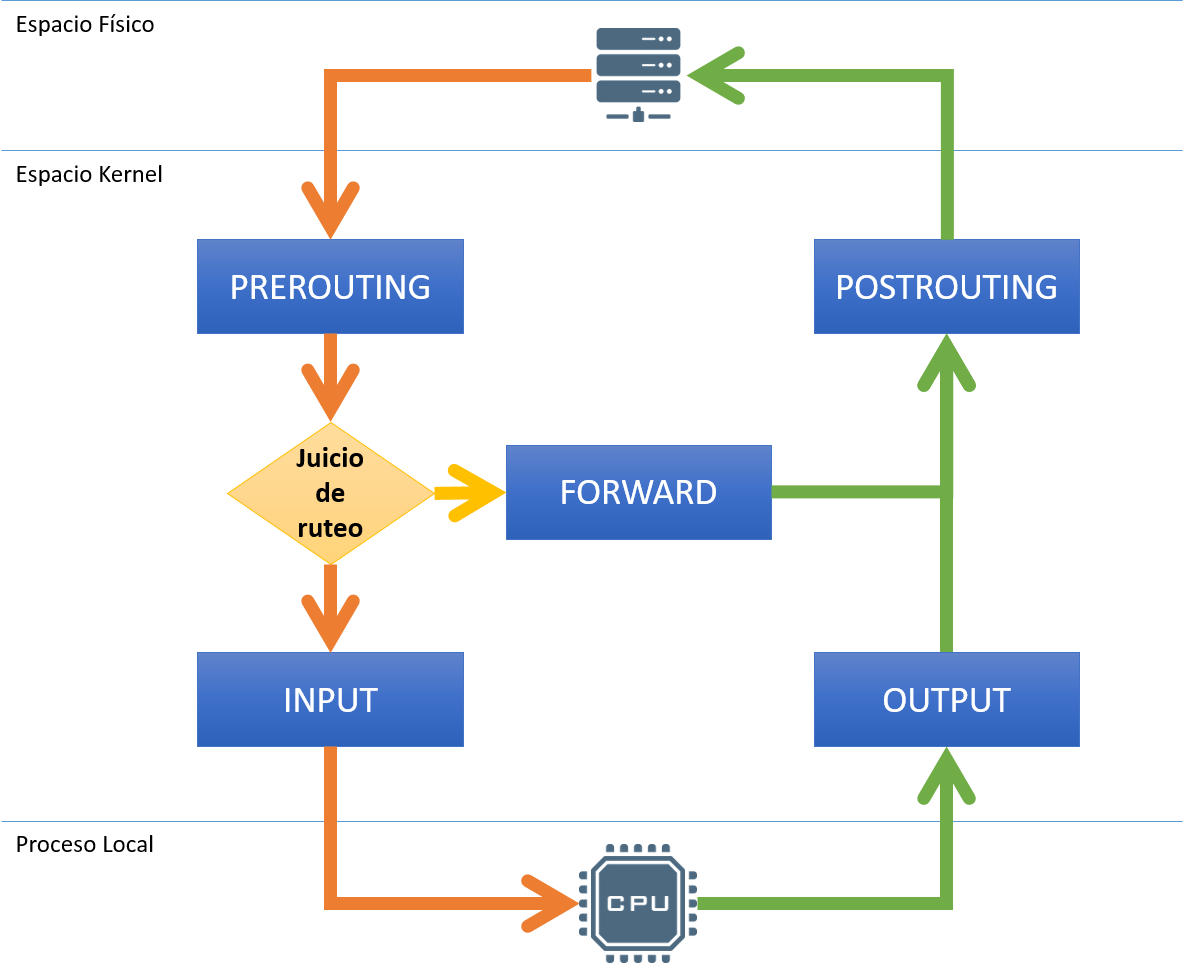
\includegraphics[scale=.5]{imagenes/netfilterArchitecture}
	\caption{Esquema de la arquitectura de interrupción disponible para la intervención de paquetes provisto por el Netfilters Framework. REVISAR EN \url{http://amsekharkernel.blogspot.cl/2012/01/what-is-netfilter-in-linux.html}}
	\label{netfilterArchitecture}
\end{figure}

\subsection{Eliminación}
La remoción de la solución desde el sistema es muy simple y se basa en que la misma es sólo un módulo del kernel, por lo tanto basta aplicar el comando \verb=rmmod= del sistema acompañado del nombre del módulo. Para una completa limpieza del módulo, es recomendable tambien limpiar los registros generados al momento de la compilación del módulo, para lo cual se puede ejecutar la directiva \verb=make clean= del archivo \verb=Makefile= provisto en la solución.

\section{Testing}
Todo.... probar en un script la cantidad de paquetes perdidos en una conexión punto a punto vs una por lo

\section{Rendimiento de la solución en la práctica}

\section{Comparación de la solución con ReusePort}

\section{Aciertos de la solución}

A raíz de los análisis anteriores, se desprenden varios aspectos rescatables de la solución implementada, obtenidos como consecuencia de satisfacer los requerimientos de operación planteados al comienzo del presente capítulo, y que diferencian neustra solución de las opciones disponibles.

Un primer elemento a destacar es el \textbf{rendimiento}. En las pruebas desarrolladas en secciones anteriores se corroboró la efectividad de la solución propuesta, comparándola con la mejor alternativa disponible: \emph{Reuseport}, de donde se concluyó que nuestra propuesta logra un comportamiento similar al de \emph{Reuseport} en terminos nominales, conservando un margen de diferencias que mantiene a \emph{Reuseport} como la opción más rápida, pero postulando nuestro desarrollo como competitivo en esa linea.

Un segundo Punto a descatar de la solución es su \textbf{equitatividad de tiempos}, una característica que lo diferencia de \emph{Reuseport} pues, nuestro diseño provee un rendimiento más homogéneo entre múltiples procesos. Ésta característica es muy interesante de resaltar pues hay aplicaciones donde es necesario garantizar un escenario altamente \emph{Fairness} y experimentalmente nuestra solución luce prometedora en ese sentido.

Otro aspecto a destacar de nuestra solución es que logra buenos rendimientos preservando los \textbf{principios de diseño del modelo OSI}. Ésta característica era fundamental de proveer pues da garantías de facil adopción de la solución en entornos con aplicaciones ya operativas sin mayores modificaciones de los mismos.

El último y más importante acierto a reconocer de neustra solución consiste en su \textbf{configurabilidad} y \textbf{extensibilidad}. El primero pues, cómo se explicó en secciones anteriores, la solución admite distintos parámetros de configuración que permiten, sin cambios del código fuente, proveer distintos modos de funcionamiento según el requerimiento de consumo y distribución que se busque. El segundo dado por la implementación misma de la solución, ello pues al ser un módulo del kernel, es facilmente modificable para añadir nuevo código fuente que permita modificar los esquemas de distribución, etapas de interceptación de paquetes, funcionamiento del framework de \emph{Netfilters}, etc.

\section{Proyecciones}
La solución planteada en la presente investigación cumple correctamente para los fines con que se postuló originalmente, basada en su satisfacción de los requerimientos especificados en la seccion previa. Sin embargo, el mismo modelo de operación que se ilustró en la solución puede ser aprovechado y extendido para ser usado en otros escenarios o contextos.

Un caso interesante consiste en extender la solución para funcionar con otros protocolos orientados a la conexión, como por ejemplo TCP. El gran problema de la solución desarrollada para con el caso de TCP es salvar correctamente la etapa de negociación inicial para establecer la conexión -El denominado \emph{Handshake} de TCP-. En este contexto, nuestra solución debe poder contemplar un mecanismo para poder hacer una correcta redistribución de paquetes para respetar la asignación apropiada entre los paquetes recibidos y las conexiones que se están llevando a cabo.

\begin{figure}[!h]
	\centering
	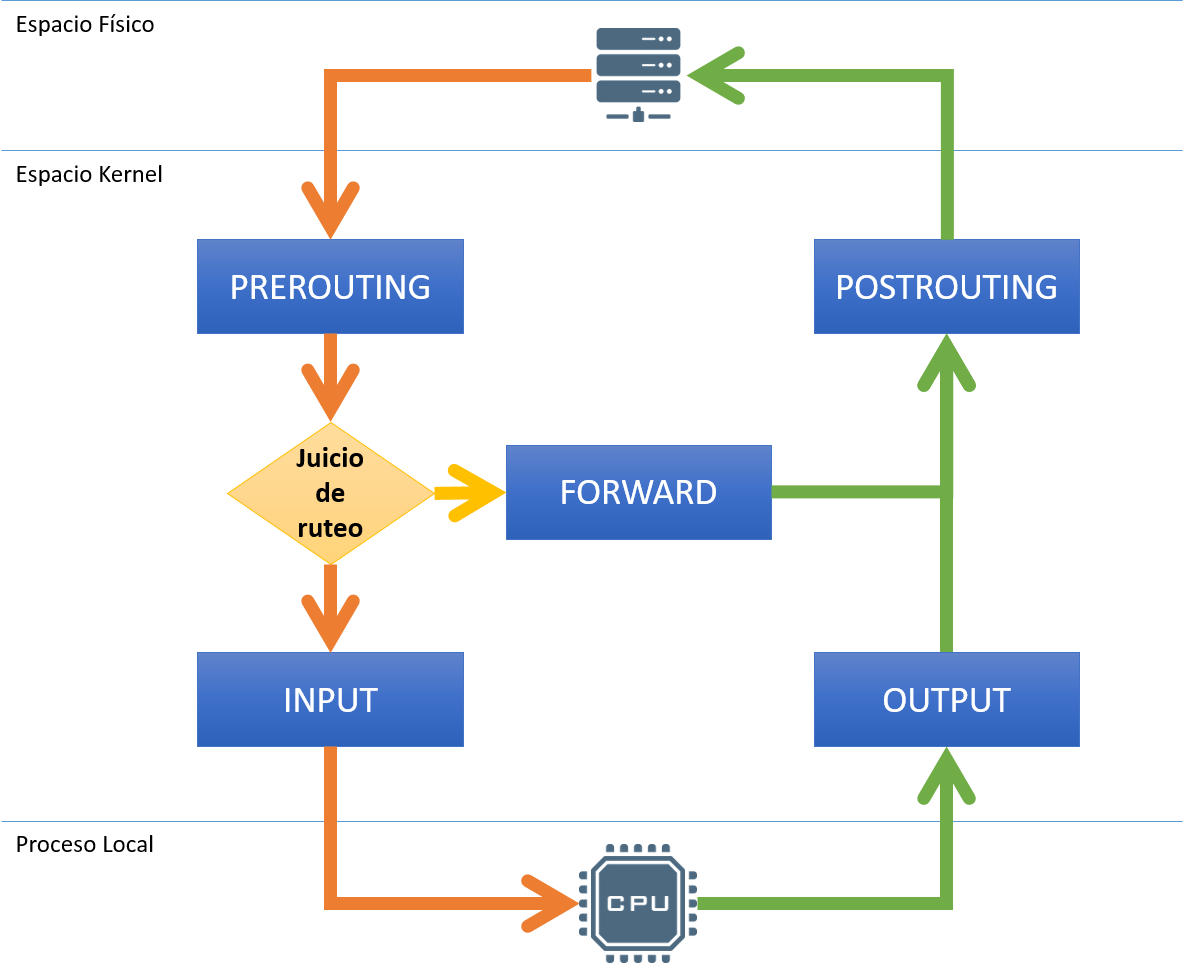
\includegraphics[scale=.2]{imagenes/netfilterArchitecture}
	\caption{Hablar del problema del handshake inicial}
	\label{netfilterArchitecture}
\end{figure}

Gracias a su buen diseño, suplir el requerimiento anterior es sencillo con nuestra solución. Basta implementar un nuevo esquema de distribución que sea conciente de la distribución de paquetes para, usando las tuplas de datos de origen/destino de cada paquete, hacer una distribución correcta entre los sockets de redirección, para que las ocnexiones sean correctas. Para ello, una solución interesante puede ser, en lugar de aplicar un criterio aleatorio o secuencial de distribución como se usó en los esquemas provistos en éste trabajo, se puede emplear una \emph{función de Hash} que use las tuplas de origen/destino de cada paquete y así, lleve un registro lógico correcto de las conexiones que están operativas sobre un mismo socket.

\begin{figure}[!h]
	\centering
	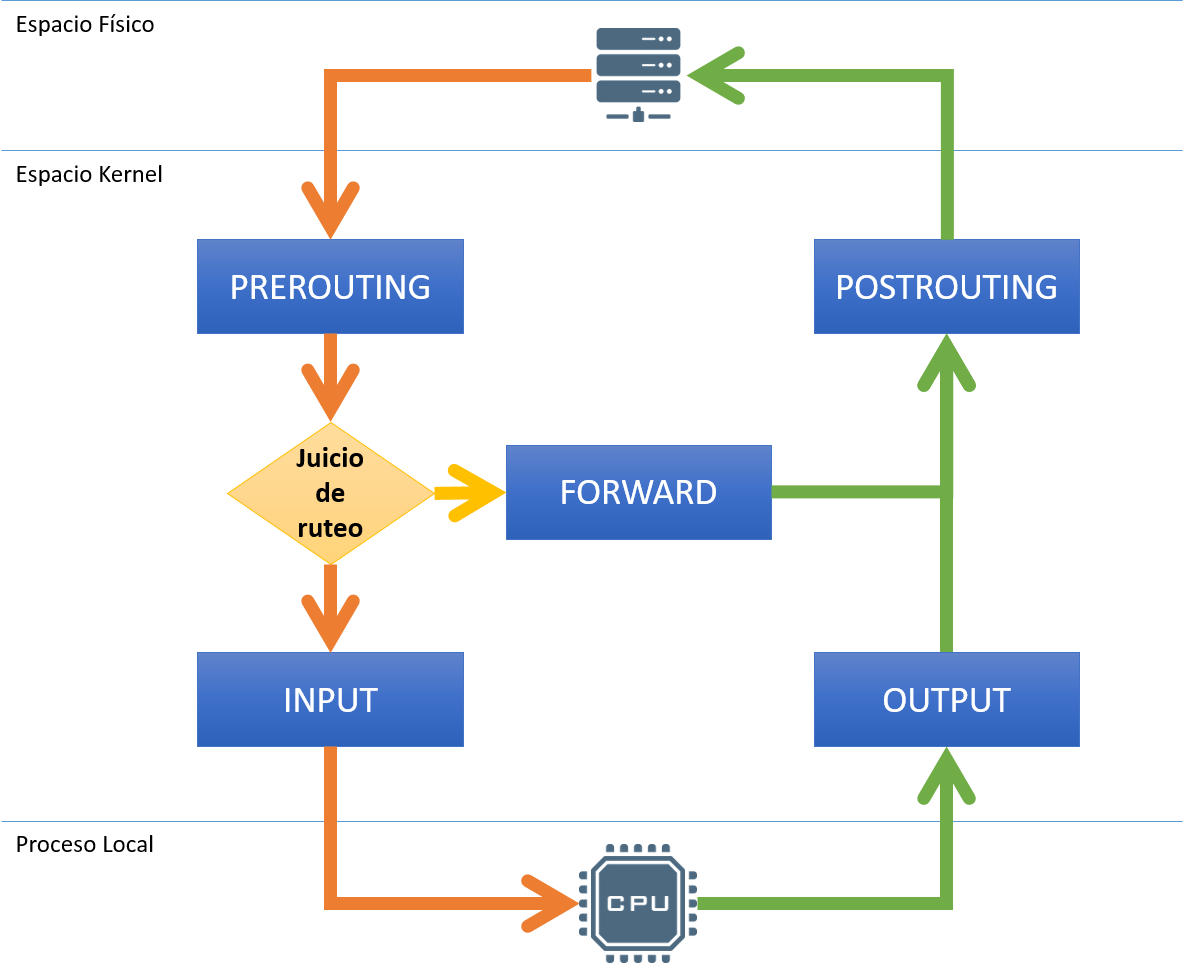
\includegraphics[scale=.2]{imagenes/netfilterArchitecture}
	\caption{Acá hablar de multiplexar un socket, un canal que permite mucha comunicacion usando multiples colores.}
	\label{netfilterArchitecture}
\end{figure}

El enfoque antes planteado es sumamente poderoso pues en la práctica, postula la capacidad de multiplexar una misma interfaz de socket del sistema, proveyéndole recepción de paquetes a un pool de otros sockets atendidos por aplicaciones independientes. Permitiendo también incrementar el número -teoricamente limitado- de sockets a usar en un sistema\footnote{Dado por la limitación de 65K puertos a usar}.

\begin{defn}[ver \cite{KAR00}] Definición definitiva $$\frac{d}{dx}\int_a^xf(y)dy=f(x).$$\end{defn}

\begin{teo}[ver \cite{KAR00}] Definición definitiva $$\frac{d}{dx}\int_a^xf(y)dy=f(x).$$\end{teo}

\begin{prop}[ver \cite{KAR00}] Definición definitiva $$\frac{d}{dx}\int_a^xf(y)dy=f(x).$$\end{prop}

\begin{obs}[ver \cite{KAR00}] Definición definitiva $$\frac{d}{dx}\int_a^xf(y)dy=f(x).$$\end{obs}

\begin{ej}[ver \cite{KAR00}] Definición definitiva $$\frac{d}{dx}\int_a^xf(y)dy=f(x).$$\end{ej}